\documentclass[a4paper, 12pt]{article}

\usepackage{arxiv}

\usepackage[T2A]{fontenc}
\usepackage[utf8]{inputenc}
\usepackage[english, russian]{babel}
% \usepackage{cmap}
\usepackage{url}
\usepackage{booktabs}
\usepackage{nicefrac}
\usepackage{microtype}
\usepackage{lipsum}
\usepackage{graphicx}
\usepackage{subfig}
\usepackage[square,sort,comma,numbers]{natbib}
\usepackage{doi}
\usepackage{multicol}
\usepackage{multirow}
\usepackage{tabularx}

\usepackage{tikz}
\usetikzlibrary{matrix}

% Algorithms
\usepackage{algpseudocode}
\usepackage{algorithm}

%% Шрифты
\usepackage{euscript} % Шрифт Евклид
\usepackage{mathrsfs} % Красивый матшрифт
\usepackage{extsizes} % Возможность сделать 14-й шрифт

\usepackage{makecell} % diaghead in a table
\usepackage{amsmath,amsfonts,amssymb,amsthm,mathtools,dsfont}
\usepackage{icomma}

\newcommand{\bz}{\mathbf{z}}
\newcommand{\bx}{\mathbf{x}}
\newcommand{\by}{\mathbf{y}}
\newcommand{\bv}{\mathbf{v}}
\newcommand{\bw}{\mathbf{w}}
\newcommand{\ba}{\mathbf{a}}
\newcommand{\bb}{\mathbf{b}}
\newcommand{\bp}{\mathbf{p}}
\newcommand{\bq}{\mathbf{q}}
\newcommand{\bt}{\mathbf{t}}
\newcommand{\bu}{\mathbf{u}}
\newcommand{\bs}{\mathbf{s}}
\newcommand{\bT}{\mathbf{T}}
\newcommand{\bX}{\mathbf{X}}
\newcommand{\bZ}{\mathbf{Z}}
\newcommand{\bS}{\mathbf{S}}
\newcommand{\bH}{\mathbf{H}}
\newcommand{\bW}{\mathbf{W}}
\newcommand{\bY}{\mathbf{Y}}
\newcommand{\bU}{\mathbf{U}}
\newcommand{\bQ}{\mathbf{Q}}
\newcommand{\bP}{\mathbf{P}}
\newcommand{\bA}{\mathbf{A}}
\newcommand{\bB}{\mathbf{B}}
\newcommand{\bC}{\mathbf{C}}
\newcommand{\bE}{\mathbf{E}}
\newcommand{\bF}{\mathbf{F}}
\newcommand{\bomega}{\boldsymbol{\omega}}
\newcommand{\btheta}{\boldsymbol{\theta}}
\newcommand{\bgamma}{\boldsymbol{\gamma}}
\newcommand{\bdelta}{\boldsymbol{\delta}}
\newcommand{\bPsi}{\boldsymbol{\Psi}}
\newcommand{\bpsi}{\boldsymbol{\psi}}
\newcommand{\bxi}{\boldsymbol{\xi}}
\newcommand{\bchi}{\boldsymbol{\chi}}
\newcommand{\bzeta}{\boldsymbol{\zeta}}
\newcommand{\blambda}{\boldsymbol{\lambda}}
\newcommand{\beps}{\boldsymbol{\varepsilon}}
\newcommand{\bZeta}{\boldsymbol{Z}}
% mathcal
\newcommand{\cX}{\mathcal{X}}
\newcommand{\cY}{\mathcal{Y}}
\newcommand{\cW}{\mathcal{W}}

\newcommand{\dH}{\mathds{H}}
\newcommand{\dR}{\mathds{R}}
% transpose
\newcommand{\T}{^{\mathsf{T}}}

% \renewcommand{\shorttitle}{\textit{arXiv} Шаблон}
\renewcommand{\epsilon}{\ensuremath{\varepsilon}}
\renewcommand{\phi}{\ensuremath{\varphi}}
\renewcommand{\kappa}{\ensuremath{\varkappa}}
\renewcommand{\le}{\ensuremath{\leqslant}}
\renewcommand{\leq}{\ensuremath{\leqslant}}
\renewcommand{\ge}{\ensuremath{\geqslant}}
\renewcommand{\geq}{\ensuremath{\geqslant}}
\renewcommand{\emptyset}{\varnothing}

\usepackage{hyperref}
% \usepackage[usenames,dvipsnames,svgnames,table,rgb]{xcolor}

\hypersetup{
	unicode=true,
	pdftitle={A template for the arxiv style},
	pdfsubject={q-bio.NC, q-bio.QM},
	pdfauthor={David S.~Hippocampus, Elias D.~Striatum},
	pdfkeywords={First keyword, Second keyword, More},
	colorlinks=true,
	linkcolor=black,        % внутренние ссылки
	citecolor=blue,         % на библиографию
	filecolor=magenta,      % на файлы
	urlcolor=blue           % на URL
}

\graphicspath{{../figures/}}

\usepackage{enumitem} % Для модификаций перечневых окружений

\theoremstyle{definition} % "Определение"
\newtheorem{definition}{Опр.}[section]

\usepackage{etoolbox}

\makeatletter
\expandafter\patchcmd\csname\string\algorithmic\endcsname{\itemsep\z@}{\itemsep=1.5mm}{}{}
\makeatother
\renewcommand{\abstractname}{Аннотация}

\title{Автоматическое выделение терминов для тематического моделирования}

\author{
    Никитина Мария Александровна \\
	\texttt{nikitina.mariia@phystech.edu} \\
	\And
	Консультант: Потапова Полина Сергеевна \\
	\texttt{potapov.polina@gmail.com}
 	\And
	Эксперт: Доктор ф-м наук, Воронцов Константин Вячеславович
}
\date{\today}

\begin{document}
\maketitle

\begin{abstract}
В данной статье рассматривается задача автоматического выделения терминов в коллекции документов. Новые научные термины появляются каждый день.
Ручное извлечение терминов с привлечением узкоспециализированных
специалистов является трудозатратным. Цель настоящей работы --- обнаружение таких терминов в коллекциях документов в автоматическом режиме. Для решения данной задачи используется метод выделения коллокаций (TopMine) в сочетании с модульной технологией тематического моделирования (с использованием библиотеки BigARTM) и современные методы, основанные на нейросетевых моделях языка. Производится сравнение рассматриваемых решений.
\end{abstract}

\keywords{тематическое моделирование \and TopMine \and BigARTM \and Automatic Term Extraction}

\section{Введение}

        Поиск научных терминов в коллекции документов вручную практически невозможен из-за слишком больших объёмов работы. Для экономии ресурсов и времени предлагается рассмотреть задачу автоматического выделения терминов. К её решению можно подойти с разных сторон. Например, использовать сочетание метода выделения коллокаций с технологией математического моделирования \citep{ElKishky2014}. \textit{Коллокация} --- слово или словосочетание, имеющее признаки синтаксически и семантически целостной единицы.

        \textit{Тематическое моделирование} --- это технология обработки естественного языка, направленная на определение тем, к которым относится текстовый документ из коллекции, и какие слова каждую тему образуют. Иначе говоря, тематическая модель осуществляет \textit{мягкую кластеризацию}, выбирая для документа кластеры-темы.

        \textit{Вероятностная тематическая модель} определяет вероятности тем в каждом документе и вероятности слов в каждой теме. Большим отличием такой модели от глубоких нейронных сетей типа BERT \citep{bert} или GPT-4 \citep{https://doi.org/10.48550/arxiv.2303.08774} является простота организации и свойство интерпретируемости в ущерб качеству предсказания вероятности появления слов в документе. Векторное представление тяжёлой нейросети всё ещё не удалось интерпретировать, в то время как тематический эмбеддинг --- это вектор вероятностей тем.

        Новизной данной статьи является сравнение этих двух подходов. В качестве нейросети использована предобученная модель BERT \citep{wolf-etal-2020-transformers}. Для построения же тематической модели требуется подбор \textit{регуляризаторов} --- критериев, учитывающих специфические особенности данных или предметной области, от подбора которых значительно зависит качество определения основных тем документов. В данной работе используется модель \textit{аддитивной регуляризации тематической модели, ARTM} \citep{vorontsov2020}. Для построения тематической модели с аддитивной регуляризацией используется библиотека BigARTM \citep{Vorontsov2015} с открытым кодом.

        Перед выполнением кластеризации необходимо выделить из коллекции документов ключевые слова и словосочетания и отбросить те, что не несут основной смысловой нагрузки. Поиск составных терминов является нетривиальной и трудоёмкой задачей. Для её решения используется метод поиска коллокаций TopMine, использующий информацию о частоте и совстречаемости слов в коллекции \citep{shatalov2019}.

        % Ещё какая-то информация про датасеты

        С учётом интерпретируемости и простоты тематическая модель является хорошей заменой нейросети. %Предшествующие исследования предлагаемого подхода показали хорошие результаты как по полноте, так и по вычислительной эффективности.
        В работе сравниваются тематическая модель и сложная нейросетевая модель, анализируется их качество для рассматриваемой задачи.

\section{Постановка задачи}

        Основная задача --- построение модели ATE (Automatic Term Extraction --- автоматическое выделение терминов) для автоматического выделения словосочетаний, являющихся терминами предметной области, в текстах научных статей. Предлагается использовать эффективные методы выделения коллокаций и тематические модели для определения «тематичности» словосочетания. Модель должна обучаться без учителя.

        Для решения поставленной задачи применяются алгоритмы поиска коллокаций TopMine \citep{ElKishky2014} с последующей фильтрацией по критерию тематичности, подбор гиперпараметров тематической модели и критерия тематичности.

        Задача называется корректно поставленной по Адамару, если её решение существует, единственно и устойчиво. В общем случае построение тематической модели – некорректно поставленная задача по Адамару, поэтому её нужно дополнить регуляризаторами. В практических задачах автоматической обработки текстов существует очень много критериев и ограничений.

        Пусть $p_{\omega d}$ -- вероятность появления терма $\omega$ в документе $d$, $\phi_{\omega t}$ -- вероятность того, что терм $\omega$ относится к теме $t$, $\theta_{td}$ -- вероятность встречи темы $t$ в документе $d$. Тогда $P = (p_{\omega d})_{W \times D}$ -- матрица частот термов в документах, $\Phi = (\phi_{\omega t})_{W \times T}$ -- матрица термов тем, $\Theta = (\theta_{td})_{T \times D}$ -- матрица тем документов. $W$, $D$, $T$ -- множества всех термов, документов и тем соответственно.
       
        Аддитивная регуляризация тематических моделей основана на максимизации логарифма правдоподобия и регуляризаторов $R_i(\Phi, \Theta)$ с неотрицательными коэффициентами регуляризации $\tau_i$, $i = 1, ..., k$ \citep{vorontsov2020}:
        \begin{equation}\label{log}
            \sum\limits_{d \in D}\sum\limits_{w \in d}n_{\omega d}\ln\sum\limits_{t \in T}\phi_{\omega t}\theta_{td} + R(\Phi, \Theta) \to \max\limits_{\Phi, \Theta}; ~~~~~ R(\Phi, \Theta) = \sum\limits_{i = 1}^k\tau_iR_i(\Phi, \Theta);
        \end{equation}
        при ограничениях неотрицательности и нормировки:
        \begin{equation}\label{lim}
            \sum\limits_{w \in W}\phi_{\omega t} = 1; ~~~ \phi_{\omega t} \geq 0; ~~~~~ \sum\limits_{t \in T}\theta_{td} = 1; ~~~ \theta_{td} \geq 0.
        \end{equation}

    Решается задача нахождения разложения $P = \Phi\Theta$ при достижении максимума. Для её решения применяется EM-алгоритм. Таким образом, основной проблемой построения тематической модели становится поиск регуляризаторов $R_i(\Phi, \Theta)$, подходящих под нашу задачу поиска терминов в коллекции документов.

\section{Анализ свойств предложенного метода}

    Для решения задачи (\ref{log})-(\ref{lim}) используется EM-алгоритм.
    
    Пусть $R_i(\Phi, \Theta)$ --непрерывно дифференцируемы. Точка локального экстремума задачи (\ref{log})-(\ref{lim}) удовлетворяет системе уравнений, если из решения удалить нулевые столбцы матриц $\Phi$ и $\Theta$ \citep{vorontsov2020}:

    \begin{equation}\label{EM1}
        p_{td\omega} = \underset{t \in T}{\text{norm}}(\phi_{\omega t}\theta_{td});
    \end{equation}
    \begin{equation}\label{EM2}
        \phi_{\omega t} = \underset{\omega \in W}{\text{norm}}\left(n_{\omega t} + \phi_{\omega t} \frac{\partial R}{\partial \phi_{\omega t}}\right); ~~~~~ n_{\omega t} = \sum\limits_{d \in D}n_{d \omega}p_{td\omega};
    \end{equation}
    \begin{equation}\label{EM3}
        \theta_{td} = \underset{t \in T}{\text{norm}}\left(n_{td} + \theta_{td} \frac{\partial R}{\partial \theta_{td}}\right); ~~~~~~~ n_{td} = \sum\limits_{\omega \in d}n_{d \omega}p_{td\omega},
    \end{equation}

    где $p_{td\omega} = p(t | d, \omega)$, 
    
    $n_{td\omega}$ -- число троек, в которых терм $\omega$ документа $d$ связан с темой $t$, 
    
    $n_{\omega t} = \sum_dn_{td\omega}$ -- число троек, в которых терм $\omega$ связан с темой $t$,

    $n_{d \omega}$ -- число вхождений терма $\omega$ в документ $d$,

    $n_{td} = \sum_{\omega}n_{td\omega}$ -- число троек, в которых терм документа $d$ связан с темой $t$.
    
    Оператор norm определяется так:

    \[\underset{i \in I}{\text{norm}}(x_i) = \frac{(x_i)_{+}}{\sum\limits_{k \in I}(x_k)_{+}}, ~~~ \text{где } (x)_{+} = \max\{0, x\}.\]

    \textit{Обобщённый регуляризатор сглаживания-разреживания}:

    \begin{equation}
        R(\Phi, \Theta) = \sum\limits_{t \in T}\sum\limits_{\omega \in W}\beta_{\omega t}\ln\phi_{\omega t} + \sum\limits_{d \in D}\sum\limits_{t \in T}\alpha_{td}\ln\theta_{td}
    \end{equation}

    Подставив этот регуляризатор в (\ref{EM2})-(\ref{EM3}), получим для M-шага:

    \begin{equation}
        \phi_{\omega t} = \underset{\omega \in W}{\text{norm}}(n_{\omega t} + \beta_{\omega t})
    \end{equation}

    \begin{equation}
        \theta_{td} = \underset{t \in T}{\text{norm}}(n_{td} + \alpha_{td})
    \end{equation}

    При положительных $\beta_{\omega t}, \alpha_{td}$ регуляризатор увеличивает правдоподобие и происходит сглаживание, при отрицательных -- уменьшение правдоподобия и разреживание.

    \textit{Декоррелирование тем}:

    \begin{equation}
        R(\Phi) = -\frac{\tau}{2}\sum\limits_{t \in T}\sum\limits_{s \in T\backslash t}\sum\limits_{\omega \in W}\phi_{\omega t}\phi_{\omega s}
    \end{equation}

    Подставив этот регуляризатор в (\ref{EM2})-(\ref{EM3}), получим для M-шага:

    \begin{equation}
        \theta_{td} = \underset{\omega \in W}{\text{norm}}(n_{\omega t} - \tau \phi_{\omega t} \sum\limits_{s \in T\backslash t}\phi_{\omega s})
    \end{equation}

    Систему (\ref{EM1})-(\ref{EM3}) можно решить методом простых итераций, чередуя E-шаг (\ref{EM1}) и M-шаг (\ref{EM2})-(\ref{EM3}).

\section{Вычислительный эксперимент}

    Для обучения модели используется открытый датасет ACL RD-TEC \citep{QZadeh2014}, в котором собраны статьи на английском языке с 1965 по 2006 год из области компьютерной лингвистики. Его описание представлено в Таблице \ref{table:Dataset}. Для проведения эксперимента из него удаляются документы, содержащие менее 20 терминов, а также плохо читаемые документы, большая часть слов в которых была сильно искажена при создании датасета. В результате получается датасет из 9,095 статей. Распределение терминов по документам представлено на Рис. \ref{fg:Dataset}.

 \begin{table}[t]%\small
    \caption{Описание датасета ACL RD-TEC}
    \label{table:Dataset}
    \centering\medskip%\tabcolsep=2pt%\small
    \begin{tabular}{| p{75 pt} | p{50 pt} | p{70 pt} | p{70 pt} | p{70 pt} |}
    \hline
        Датасет
            & Год
            & Количество документов
            & Количество слов
            & Количество терминов \\ \hline
        ACL RD-TEC
            & 2014
            & 10,922
            & 36,729,513
            & 82,000 \\
    \hline
    \end{tabular}
\end{table}

\begin{figure}[!ht]
    \subfloat[Все термины]{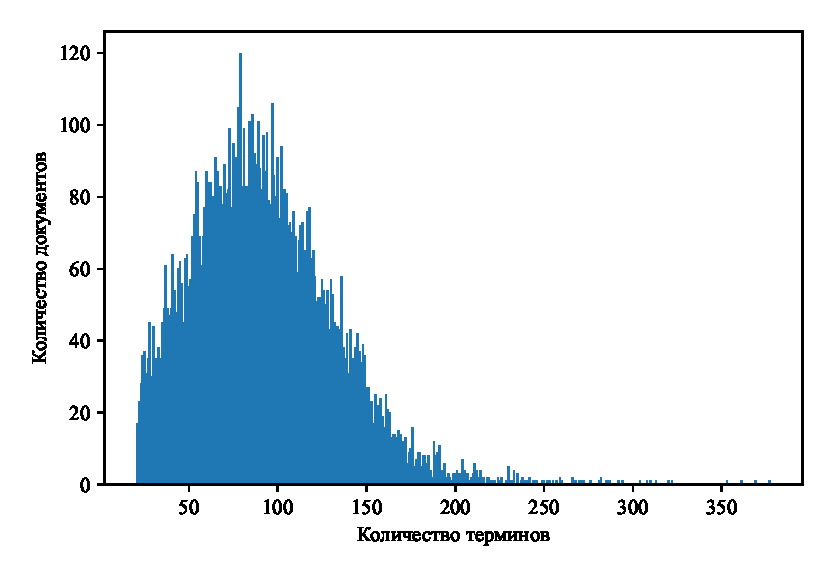
\includegraphics[scale = 0.6]{Pictures/Statistics.eps}}
    \subfloat[Термины, состоящие из одного слова]{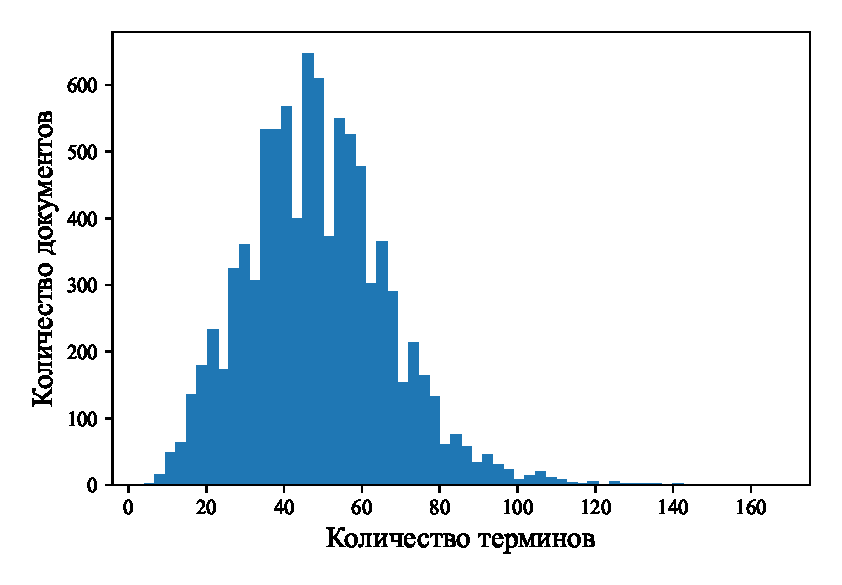
\includegraphics[scale = 0.6]{Pictures/Statistics_1.eps}}
    \caption{Распределение терминов по документам}
    \label{fg:Dataset}
\end{figure}

    Документы представлены в текстовом формате и были получены путём считывания текста из pdf-файлов. Для проведения первого эксперимента из статей удаляются числа, заголовки и ссылки на литературу, затем эксперимент разделяется на два направления: выделение терминов с помощью библиотеки BigARTM и поиск кандидатов в термины с помощью TopMine. Поиск терминов сначала осуществляется в предположении, что они состоят из одного слова.

\subsection{BigARTM}
    Для использования BigARTM необходимо привести слова к нормальной форме. Так как датасет состоит из статей, написанных на английском языке, для этого используется \textit{стемминг} --- отбрасывание окончаний и других изменяемых частей слова. Также для улучшения результата из текста выбрасываются стоп-слова, например: <<the>>, <<a>>, <<however>>. Затем полученные документы собираются в файл формата Vowpal Wabbit, который уже обрабатывается с помощью библиотеки BigARTM.
    
    Для подбора подходящих гиперпараметров эксперимент запускается с различными комбинациями гиперпараметров \textit{сглаживания}, \textit{разреживания} и \textit{декоррелирования}. Подробное их описание есть в \citep{Vorontsov2014}. Сглаживание применяется для фоновых тем, куда собираются слова, не имеющие определённой темы. Сами по себе они не несут никакой смысловой нагрузки. В эксперименте выбрано 2 фоновые темы. Разреживание применяется для предметных тем. В отличие от гиперпараметра сглаживания влияние разреживания рекомендуется увеличивать постепенно в процессе обучения модели. Декорреляция отвечает за степень различия между темами.

    Результат работы алгоритма --- матрица $\Phi$, состоящая из вероятностей принадлежности некоторого терма к некоторой теме. Следует выделить из этих термов термины. В большинстве случаев термин отличается от обычного слова или словосочетания тем, что имеет большую вероятность пояления только в 1-2 темах. Таким образом выделяются все кандидаты в термины для коллекции документов.

\subsection{TopMine}
    Вторая часть эксперимента --- выделение коллокаций с помощью TopMine. Данный алгоритм выделяет термины, основываясь на частоте появления слов в документе. После обработки документов без чисел, заголовков и литературы получается список кандидатов в термины для каждого документа отдельно.

    После пересечения списка терминов, полученных с помощью BigARTM, с коллокациями, выделенными алгоритмом TopMine, получается окончательный список терминов для каждого документа.

\subsection{Анализ ошибки}
    Для анализа ошибки используются Precision -- точность, Recall -- полнота, а также F1 -- их среднее гармоническое:

    \begin{equation}
        \text{Precision} = \frac{TP}{TP + FP}; ~~~ \text{Recall} = \frac{TP}{TP + FN};
    \end{equation}
    \begin{equation}
        \text{F1} = 2 \cdot \frac{\text{Precision} \cdot \text{Recall}}{\text{Precision} + \text{Recall}},
    \end{equation}

    \noindentгде $TP$ -- истинно-положительное решение, $FP$ -- ложноположительное решение, $FN$ -- ложноотрицательное решение.

    В Таблице \ref{table:Res_1} представлены некоторые результаты (от худшего к лучшему), полученные без выделения фоновых тем. В таблице \ref{table:Res_1} представлены результаты, полученные с выделением 2 фоновых тем.

    Кол-во тем -- количество тем, на которые разбиваются слова в датасете. Во второй таблице количество тем везде равно 150. Их меньше, чем в первой, из-за выделения фоновых тем. Это удобно, так как размер выходной матрицы вероятностей $\Phi$ сильно уменьшается.

    $\tau_{dec}$ -- значение коэффициента декорреляции. В случае выделения фоновых тем он задаётся отдельно для предметных и отдельно для фоновых тем.

    $\tau_{\Phi}$ -- значение коэффициента сглаживания-разреживания матрицы $\Phi$. Во второй таблице представлено его значение для предметных и фоновых тем отдельно.

    $\tau_{\Theta}$ -- значение коэффициента сглаживания-разреживания матрицы $\Theta$. Во второй таблице представлено его значение для предметных и фоновых тем отдельно.

    Порог -- пороговое значение вероятности для отбора кандидатов в термины.

    Кол-во тем для термина -- разрешённое количество тем, для которых термин имеет большую вероятность. Заметно, что при наличии выделения фоновых тем для лучшего результата требуется меньшее значение этого параметра.

    \begin{table}[!ht]
    \caption{Результаты работы алгоритма для нахождения терминов, состоящих из одного слова, без выделения фоновых тем}
    \label{table:Res_1}
    \centering\medskip
    \begin{tabular}{|l|p{40 pt}|l|l|l|l|p{50 pt}|l|l|l|}
    \hline
        N & Кол-во тем & $\tau_{dec}$ & $\tau_{\Phi}$ & $\tau_{\Theta}$ & Порог & Кол-во тем для термина & Precision & Recall & F1 \\ \hline
        1 & 200 & 0.025 & 0.025 & 0.025 & 1.00E-04 & 1 — 2 & 0.023 & 0.031 & 0.026 \\ \hline
        2 & 200 & 0.025 & 0.025 & 0.025 & 5.00E-04 & 1 — 4 & 0.058 & 0.176 & 0.087 \\ \hline
        3 & 200 & 0.025 & 0.025 & 0.025 & 7.00E-04 & 1 — 5 & 0.078 & 0.270 & 0.121 \\ \hline
        4 & 200 & 0.025 & 0.025 & 0.025 & 1.00E-03 & 1 — 6 & 0.098 & 0.354 & 0.154 \\ \hline
        5 & 200 & 0.025 & 0.025 & -0.25 & 1.00E-03 & 1 — 6 & 0.091 & 0.332 & 0.142 \\ \hline
        6 & 200 & 0.025 & 0.100 & 0.025 & 5.00E-04 & 1 — 4 & 0.104 & 0.345 & 0.160 \\ \hline
        \textbf{7} & \textbf{200} & \textbf{0.025} & \textbf{0.100} & \textbf{0.025} & \textbf{1.00E-03} & \textbf{1 — 6} & \textbf{0.156} & \textbf{0.432} & \textbf{0.229} \\ \hline
        8 & 200 & 0.025 & 0.100 & 0.100 & 1.00E-03 & 1 — 6 & 0.155 & 0.432 & 0.228 \\ \hline

    \end{tabular}
\end{table}

\begin{table}[!ht]
    \caption{Результаты работы алгоритма для нахождения терминов, состоящих из одного слова, с выделением фоновых тем}
    \label{table:Res_2}
    \centering\medskip
    \begin{tabular}{|l|l|l|l|l|l|l|p{50 pt}|l|l|l|}
    \hline
        N & $\tau_{dec}$ & $\tau_{\Phi}$ & $\tau_{\Phi}$ (фон) & $\tau_{\Theta}$  & $\tau_{\Theta}$ (фон) & Порог & Кол-во тем для термина & Precision & Recall & F1 \\ \hline
        1 & 0.1 & -0.1 & 0.1 & 0.1 & -0.1 & 0.01 & 1 — 4 & 0.204 & 0.358 & 0.260 \\ \hline
        2 & 0.1 & -0.1 & 0.1 & 0.1 & -0.1 & 0.3 & 1 — 2 & 0.553 & 0.096 & 0.164 \\ \hline
        3 & 0.1 & -0.1 & 0.2 & 0.1 & -0.1 & 0.05 & 1 — 4 & 0.458 & 0.213 & 0.290 \\ \hline
        4 & 0.01 & -0.1 & 0.1 & -0.1 & 0.2 & 0.03 & 1 — 2 & 0.395  & 0.255 & 0.310 \\ \hline
        5 & 0.01 & -0.1 & 0.2 & -0.1 & 0.2 & 0.03 & 1 — 2 & 0.407 & 0.263 & 0.319 \\ \hline
        6 & 0.01 & -0.1 & 0.05 & -0.1 & 0.2 & 0.03 & 1 — 2 & 0.389 & 0.240 & 0.297 \\ \hline
        7 & 0.01 & -0.2 & 0.1 & -0.1 & 0.2 & 0.03 & 1 — 2 & 0.363 & 0.266 & 0.307 \\ \hline
        8 & 0.01 & -0.2 & 0.2 & -0.1 & 0.2 & 0.03 & 1 — 2 & 0.365 & 0.268 & 0.309 \\ \hline
        9 & 0.01 & -0.2 & 0.05 & -0.1 & 0.2 & 0.03 & 1 — 2 & 0.369 & 0.270 & 0.312 \\ \hline
        10 & 0.01 & -0.05 & 0.1 & -0.1 & 0.2 & 0.03 & 1 — 2 & 0.415 & 0.243 & 0.306 \\ \hline
        11 & 0.01 & -0.05 & 0.2 & -0.1 & 0.2 & 0.03 & 1 — 2 & 0.417 & 0.254 & 0.316 \\ \hline
        12 & 0.01 & -0.05 & 0.05 & -0.1 & 0.2 & 0.03 & 1 — 2 & 0.394 & 0.230 & 0.291 \\ \hline
        \textbf{13} & \textbf{0.01} & \textbf{-0.1} & \textbf{0.2} & \textbf{-0.1} & \textbf{0.2} & \textbf{0.03} & \textbf{1 — 4} & \textbf{0.413} & \textbf{0.286} & \textbf{0.338} \\ \hline
        \textbf{14} & \textbf{0.01} & \textbf{-0.1} & \textbf{0.2} & \textbf{-0.1} & \textbf{0.1} & \textbf{0.03} & \textbf{1 — 4} & \textbf{0.413} & \textbf{0.286} & \textbf{0.338} \\ \hline
        \textbf{15} & \textbf{0.01} & \textbf{-0.1} & \textbf{0.2} & \textbf{-0.2} & \textbf{0.1} & \textbf{0.03} & \textbf{1 — 4} & \textbf{0.426} & \textbf{0.281} & \textbf{0.338} \\ \hline
        \textbf{16} & \textbf{0.01} & \textbf{-0.1} & \textbf{0.2} & \textbf{-0.2} & \textbf{0.2} & \textbf{0.03} & \textbf{1 — 4} & \textbf{0.424} & \textbf{0.281} & \textbf{0.338} \\ \hline
        \textbf{17} & \textbf{0.01} & \textbf{-0.1} & \textbf{0.2} & \textbf{-0.1} & \textbf{0.05} & \textbf{0.03} & \textbf{1 — 4} & \textbf{0.424} & \textbf{0.281} & \textbf{0.338} \\ \hline
        18 & 0.01 & -0.1 & 0.2 & -0.05 & 0.1 & 0.03 & 1 — 4 & 0.402 & 0.276 & 0.327 \\ \hline
        19 & 0.01 & -0.1 & 0.2 & -0.05 & 0.2 & 0.03 & 1 — 4 & 0.400 & 0.276 & 0.327 \\ \hline
        20 & 0.01 & -0.1 & 0.2 & -0.05 & 0.05 & 0.03 & 1 — 4 & 0.402 & 0.276 & 0.327 \\ \hline
        21 & 0.1 & -0.1 & 0.1 & -0.1 & 0.1 & 0.03 & 1 — 4 & 0.498 & 0.229 & 0.313 \\
        \hline
    \end{tabular}
\end{table}

    Лучший результат, полученый при вариации гиперпараметров: F1$= 0.338$. Отметим отдельно результат работы алгоритма TopMine без использования модульного тематического моделирования -- таблица \ref{table:TopMine}. Параметр F1 в 3 раза меньше, чем у лучшего результата объединения двух алгоритмов.

    \begin{table}[!ht]
    \caption{Результаты работы алгоритма TopMine}
    \label{table:TopMine}
    \centering\medskip
    \begin{tabular}{|l|l|l|}
    \hline
        Precision & Recall & F1 \\ \hline
        0.063 & 0.946 & 0.117 \\
        \hline
    \end{tabular}
\end{table}

    Пример зависимости значения метрики F1 от значения гиперпараметров приведён на графике \ref{fg:Res}.


    \begin{figure}[!ht]
    \subfloat[Зависимость F1 от $\tau_{\Phi}$ (фон)]{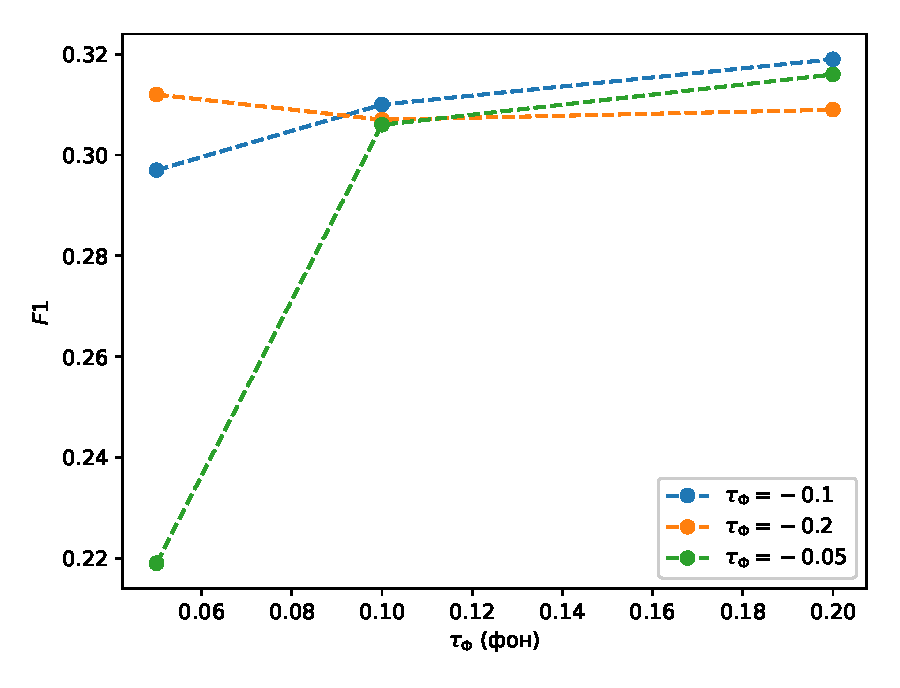
\includegraphics[scale = 0.6]{Pictures/Results.eps}}
    \subfloat[Зависимость F1 от $\tau_{\Phi}$]{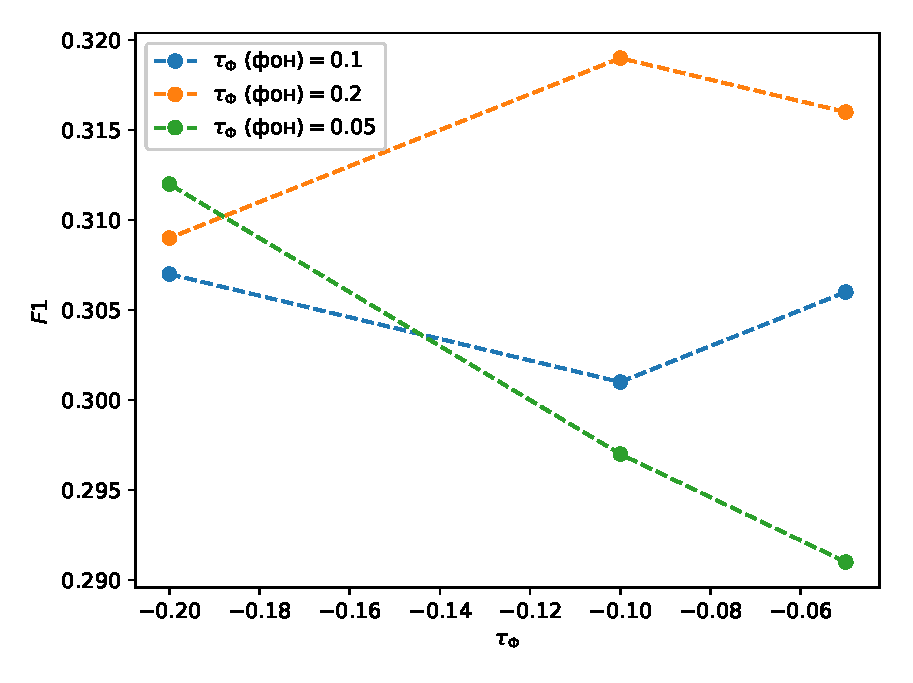
\includegraphics[scale = 0.6]{Pictures/Results_1.eps}}
    \caption{Зависимость F1 от $\tau_{\Phi}$ (фон) и $\tau_{\Phi}$ при $\tau_{\Theta} = -0.1$, $\tau_{\Theta}$ (фон) $=0.2$}
    \label{fg:Res}
    \end{figure}

\section{Заключение}

\bibliographystyle{plain}
\bibliography{references.bib}

\end{document}
